\documentclass{./../../Latex/tests}
\begin{document}
\thispagestyle{plain}
\myheader{Sample Final Exam Solutions}
\rhead{Sample Final Exam Solutions}

\vspace{0.5em}
\testHeader{110}{40}

%%%%%%%%%%%%%%%%%%%%%%%%%%%%%%%%%%%%%%%%% Question 1
\begin{enumerate}
\item (5 pts) Answer the following questions. (1 pt each)
\begin{enumerate}
\item What is the inverse of the function $f(x)= 4x + 6$? \\
$$ f^{-1}(x) = g(x) = \frac{x-6}{4}  $$

\vspace{1em}
\item  Find the intersection of the following sets:
$$ A = \{x: x>0 \} \quad \quad B = \{x: x\text{ is an even number} \} $$ 
$$ A \cap B = \{2, 4, 6, \hdots \}  $$ 

\vspace{1em}
\item  The inverse of a $4\times 4$ matrix $A$ exists if
\begin{itemize}
	\item[$\square$] The determinant of $A$ is 0 
	\item[$\text{\rlap{$\checkmark$}}\square$] The determinant of $A$ is not 0 
	\item[$\text{\rlap{$\checkmark$}}\square$] Rank of $A$ is 4
	\item[$\square$] Rank of $A$ is 0
	\item[$\text{\rlap{$\checkmark$}}\square$] All rows of $A$ are linearly independent
\end{itemize}  
\textit{Select all that apply.}

\vspace{1em}
\item  Is the function $y=|x-1|$ differentiable at $x=1$? 
\begin{itemize}
	\item[$\square$] Yes. 
	\item[$\text{\rlap{$\checkmark$}}\square$] No.
	\item[$\square$] Can't say. \\~\\
\end{itemize}  
\item The function $f(K,L) = K^{\alpha} L^{1-\alpha}$ is:
\begin{itemize}
  \item[$\square$] Homogeneous of degree 0
  \item[$\text{\rlap{$\checkmark$}}\square$] Homogeneous of degree 1
  \item[$\square$] Not homogeneous 
  \item[$\square$] Homogeneous but cannot say of what degree \\~\\
\end{itemize}

% Part (f)
\newpage
\item The following function is:
\begin{center}
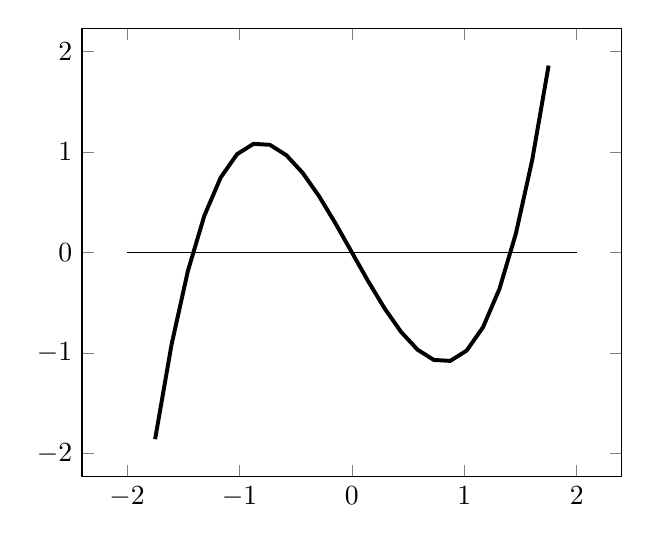
\begin{tikzpicture}
\begin{axis}[]
\addplot[color=black, line width=0.5mm, domain=-1.75:1.75] {x^3-2*x};
\addplot[domain=-2:2] {0};
\end{axis}
\end{tikzpicture} 
\end{center}
\begin{itemize}
  \item[$\square$] Quasiconcave
  \item[$\square$] Strictly quasiconcave
  \item[$\square$] Quasiconvex
  \item[$\text{\rlap{$\checkmark$}}\square$] None of the above \\~\\
\end{itemize} 
\end{enumerate} 

%%%%%%%%%%%%%%%%%%%%%%%%%%%%%%%%%%%%%%%%% Question 2
\item (5 pts) Consider a single-variable function:
 $$ y = f(x) $$
 In class, we learnt that at any local maximum or minimum, we must have that, 
 $$ f'(x^*) = 0 $$
 In addition, a sufficient condition for a critical point $x^*$ to be a local maximizer is:
 $$ f''(x^*) <0 $$ 
 \begin{enumerate}
  \item (2 pts) Why can't we have a maximum or minimum at a point where $f'(x)>0$ or $f'(x)<0$? \\~\\
  A point where $f'(x)>0$ or $f'(x)<0$ cannot be a local maximum or minimum because the value of the function will change in the neighborhood of such a point. For example, if $f'(x^*)>0$, then increasing $x$ slightly above $x^*$ will lead to an increase in the value of the function, so $x^*$ cannot be a local maximum. Similarly, decreasing $x$ slightly below $x^*$ will lead to a decline in the value of the function, so $x^*$ cannot be a local minimum as well. \\~\\
  \item (2 pts) Why is $f''(x) <0$ a sufficient condition for a critical point to be a maximizer? \\~\\
If $x^*$ is a critical point, that is $f'(x^*)=0$, and $f''(x^*)<0$, we can conclude that $x^*$ is a local maximizer. This is because $f''(x^*)<0$ implies that $f'(x)$ is decreasing around $x^*$, and since $f'(x^*)=0$, the sign of $f'(x)$ flips from positive to negative as we move from left to right of $x^*$. Since $f'(x)>0$ indicates that $f(x)$ is increasing and $f'(x)<0$ indicates that $f(x)$ is decreasing, it follows that $f(x)$ is increasing as we approach $x^*$ and decreasing as we move away from it. Therefore, $x^*$ corresponds to a peak in the function. \\~\\
  \item (1 pt) If $f$ is a strictly concave function, can we have two critical points, i.e., two distinct values of $x$ such that $f'(x_1) = f'(x_2) = 0$? \\~\\
No, if $f$ is a strictly concave function, it cannot have two distinct critical points. This is due to the fact that $f''(x)<0$ for all $x$ in the domain of $f$, implying that $f'(x)$ is strictly decreasing. As a result, $f'(x)$ can only be zero at one point.
\end{enumerate}


\newpage
%%%%%%%%%%%%%%%%%%%%%%%%%%%%%%%%%%%%%%%%% Question 3
\item (5 pts) Prove the following statements:
\begin{enumerate}
\item (2 pts)  $ \sum_{i=1}^2 3 (x_i +1) = 3 \sum_{i=1}^2 x_i + 6 $ 
\begin{align*}
	\sum_{i=1}^2 3 (x_i +1) &= 3(x_1+1) + 3(x_2+1) \\
	& = 3x_1 + 3 + 3x_2 + 3 \\
	& = 3(x_1+x_2) + 6 \\
	& = 3 \sum_{i=1}^2 x_i + 6 \\
\end{align*}
\item (3 pts)  Given the following production function: 
$$ Q = f(K, L) = A K^{\alpha} L^{\beta} $$
The partial elasticity of output with respect to capital $K$ and labor $L$ is $\alpha$ and $\beta$, respectively. \\

Elasticity of output w.r.t. capital:
$$ \varepsilon_{QK} = \frac{\partial Q}{\partial K}\cdot \frac{K}{Q} = \alpha A K^{\alpha-1} L^{\beta}\cdot \frac{K}{A K^{\alpha} L^{\beta}} = \alpha $$

Elasticity of output w.r.t. labor:
$$ \varepsilon_{QL} = \frac{\partial Q}{\partial L}\cdot \frac{L}{Q} = \beta A K^{\alpha} L^{\beta-1}\cdot \frac{L}{A K^{\alpha} L^{\beta}} = \beta $$
\end{enumerate} 

\vspace{1cm}

\newpage
%%%%%%%%%%%%%%%%%%%%%%%%%%%%%%%%%%%%%%%%% Question 4
\item (6 pts) \textit{Consider the following system of equations:
}\begin{align*}
x_1 + 2 x_2 = 6 \\
3 x_1 + x_2 = 3 \\
\end{align*}
\begin{enumerate}
  \item (1 pt) \textit{Write this system of equations in matrix format i.e., $$ Av=b $$
  What is $A$, $v$, and $b$ equal to?} \\
  
  $A=\left[\begin{array}{rrr}1 & 2  \\ 3 & 1  \end{array}\right] \quad v=\left[\begin{array}{l}x_1 \\ x_2 \end{array}\right] \quad b=\left[\begin{array}{c}6 \\ 3 \end{array}\right]$ \\~\\
   \item (2 pts) \textit{Calculate the inverse of $A$. } \\
   
   $$ A^{-1} = \frac{1}{|A|} \left[ \begin{array}{cc} a_{22} & -a_{12} \\ -a_{21} &  a_{11}  \end{array} \right] = -\frac{1}{5} \left[ \begin{array}{cc} 1 & -2 \\ -3 &  1  \end{array} \right]  $$ \\
   
 
  \item (1 pts) \textit{If you premultiply $A^{-1}$ on both sides of the equation $ Av=b $, you should be able to derive an expression to solve for $v$. Write down this expression. } \\

  Premultiplying by $A^{-1}$ :
$$
A^{-1} A v=A^{-1} b 
$$
Since $A^{-1} A=I$, we have  $v^*=A^{-1} b$. \\


  
  \item (2 pts) \textit{Using the expression in $(c)$ solve for $v^*$. } 

$$
\begin{aligned}
v^{*} &=-\frac{1}{5} \left[ \begin{array}{cc} 1 & -2 \\ -3 &  1  \end{array} \right] \left[\begin{array}{c}6 \\ 3 \end{array}\right] = -\frac{1}{5} \left[ \begin{array}{c} 0 \\ -18+3  \end{array} \right] =  \left[ \begin{array}{c} 0 \\ 3  \end{array} \right]
\end{aligned}
$$
\end{enumerate}

\newpage
%%%%%%%%%%%%%%%%%%%%%%%%%%%%%%%%%%%%%%%%% Question 5
\item (14 pts) You are given the following inter-temporal utility function:
\begin{align}
	U = U(c_1, c_2) =  \ln c_1 + \beta \ln c_2
\end{align}
where $c_1$ and $c_2$ is consumption in period 1 and 2, respectively. $0<\beta<1$ is the rate at which you discount the future and it measures your impatient. You earn income $y_1>0$ in period 1 and income $y_2>0$ in period 2. Any of the income you save $s$ in period 1 earns interest $r>0$. So, $$ c_1 + s = y_1, \quad \quad c_2 = y_2 + (1+r) s $$
Combining these constraints:
$$ c_1 + \frac{1}{1+r} c_2 = y_1 + \frac{1}{1+r} y_2 $$
Let the present-discounted income be denoted by $m$, such that:
$$ m = y_1 + \frac{1}{1+r} y_2 $$

\vspace{1em}
You want to choose $c_1$ and $c_2$ to maximize utility $U(c_1, c_2)$ in equation (1) subject to the constraint:
 \begin{align} c_1 + \frac{1}{1+r} c_2 = m \end{align}

\begin{enumerate}
	\item (2 pts) Write down the Lagrangian function corresponding to this maximization problem. 
	$$ L(c_1, c_2, \lambda) = \ln c_1 + \beta \ln c_2 + \lambda\left(m- c_1 - \frac{1}{1+r} c_2 \right) $$
	\item (3 pts) Write down the first-order conditions for a critical point. 
	\begin{align}
		\frac{\partial L}{\partial c_1}&=\frac{1}{c^*_1}-\lambda^*=0 \\
		\frac{\partial L}{\partial c_2}&=\frac{\beta}{c^*_2}-\frac{\lambda^*}{1+r}=0 \\
		\frac{\partial L}{\partial \lambda}&=m- c^*_1 - \frac{1}{1+r} c^*_2=0
	\end{align}
	\item (2 pts) Using the first order conditions in (b), show that the optimal consumption $c_1^*$ and $c_2^*$ and the Lagrange multiplier $\lambda^*$ are given by:
	$$ c_1^* =\frac{m}{1+\beta}, \quad  c_2^* = \frac{\beta m(1+r)}{1+\beta}, \quad \lambda^* = \frac{1+\beta}{m} $$

	Note that from (3), $\lambda^*=1/c_1^*$, plugging this in (4), we get:
	$$ c_2^* = \beta(1+r)c_1^*  $$
	Plugging this expression for $ c_2^*$ in (5):
	$$ c_1^* + \frac{1}{1+r}\beta(1+r)c_1^* = m \rightarrow c_1^* =\frac{m}{1+\beta}  $$
	In which case,
	$$ c_2^* = \beta(1+r)c_1^* = \frac{\beta m(1+r)}{1+\beta}    $$
	Finally, since $\lambda^*=1/c_1^*$,
	$$\lambda^*=\frac{1}{c_1^*} = \frac{1+\beta}{m} $$
	\item (1 pt) Here, $U(c_1, c_2)$ is a strictly quasiconcave function. Is this sufficient to conclude that the $c_1^*$ and $c_2^*$ we found in (c) characterize a global maximum? \\
	Answer: Yes \\
	\item (2 pts) How does the optimal consumption in period 1 and 2 change due to an increase in $m$? Calculate $\partial c_1^*/\partial m$ and $\partial c_2^*/\partial m$ to answer your question. 
	
	$$\frac{\partial c_1^*}{\partial m} = \frac{1}{1+\beta}>0, \quad \quad \frac{\partial c_2^*}{\partial m} = \frac{\beta(1+r)}{1+\beta}>0 $$ 
	Since $\beta>0, r>0$, both $\partial c_1^*/\partial m$ and $\partial c_2^*/\partial m$ are positive and hence optimal consumption increases in both periods due to an increase in $m$. In particular, $c_1^*$ increases by $1/(1+\beta)$ for a one unit increase in $m$. While, $c_2^*$ increases by $\beta(1+r)/(1+\beta)$ for a one unit increase in $m$.
	\item (1 pt) If $r=0$, using your expressions for $\partial c_1^*/\partial m$ and $\partial c_2^*/\partial m$, answer whether optimal consumption in period 1 increases by more or less than consumption in period 2 in response to a change in $m$?
	When $r=0$, 
	$$\frac{\partial c_1^*}{\partial m} = \frac{1}{1+\beta}>\frac{\beta}{1+\beta}=\frac{\partial c_2^*}{\partial m} $$ 
	Since $\beta<1$ (consumption in the future is discounted), when the interest rate $r=0$, optimal consumption in period 2 increases by less relative to period 1 due to a one unit increase in $m$. 
	\item (2 pts) How does optimal consumption in period 1 change due to an increase in the interest rate $r$? \\
	
	Note that here, $$ m = y_1 + \frac{y_2}{1+r}  $$
	So to calculate $\partial c_1^*/\partial r$, you need to use the chain-rule as follows:
	$$ \frac{\partial c_1^*}{\partial r} = \frac{\partial c_1^*}{\partial m}\cdot \frac{\partial m}{\partial r} = \frac{1}{1+\beta}\cdot\frac{-y_2}{(1+r)^2} <0 $$
	So optimal consumption in period 1 decreases due to an increase in interest rate $r$. 
	\end{enumerate}

\end{enumerate}
\end{document}